\chapter{Đối xứng và các định luật bảo toàn}

\lectureoverview{Nguyên lý tác dụng dừng và các phương trình Euler--Lagrange là một nửa cốt lõi của cơ học cổ điển; dạng Hamilton là nửa còn lại. Ở đây chúng ta phát triển nửa thứ nhất đủ xa để bộc lộ một khuôn mẫu sâu sắc: mọi đối xứng liên tục của một Lagrangian đều sinh ra một đại lượng bảo toàn. Chúng ta sẽ nhận ra khuôn mẫu ấy trong các phép tịnh tiến và quay, chứng minh nó cho một phép biến đổi vô cùng bé tổng quát, rồi xem xét cẩn thận những chỗ lập luận có áp dụng và không áp dụng.}

\section{Phần toán học tối thiểu giải thích được vật lý}

Những ký hiệu đã có sẵn trên bảng có thể trông hơi giống phương trình Schrödinger, nhưng đó không phải chủ đề của tối nay. Chủ đề là đối xứng và bảo toàn. Không có cách trung thực nào để giải thích mối liên hệ của chúng mà không dùng phương trình. Các phương trình là sơ cấp; điều quan trọng là sắp xếp chúng sao cho cấu trúc trở nên nhìn thấy được. Scientific American có thể nêu tên kết quả, nhưng ở đây ta muốn lượng toán học tối thiểu cần thiết để suy ra nó theo cách các nhà vật lý vẫn làm.

Hãy đưa vào một tham số nhỏ \(\epsilon\). Ta giữ lại các hạng tỉ lệ với \(\epsilon\) và bỏ qua \(O(\epsilon^2)\). Đây là cách viết tắt cho một lập luận lấy giới hạn, chứ không phải khẳng định rằng một số thực khác không theo nghĩa đen lại có bình phương bằng không. Với một hàm thông thường \(f(x,y)\), \begin{equation}
  \delta f
  =\frac{\partial f}{\partial x}\,\delta x
   +\frac{\partial f}{\partial y}\,\delta y
   +O(\epsilon^2),
  \label{eq:first-variation-f}
\end{equation} trong đó cả \(\delta x\) lẫn \(\delta y\) đều tỉ lệ với \(\epsilon\). Ký hiệu \(\delta f\) có nghĩa là độ biến thiên của \(f\), chứ không phải tích của một số gọi là \(\delta\) với \(f\). Một điểm dừng thỏa mãn \begin{equation}
  \delta f=0
  \qquad\hbox{to first order.}
  \label{eq:stationary-f}
\end{equation}

Đối với một quỹ đạo cơ học \(q_i(t)\), đại lượng tương tự là tác dụng \begin{equation}
  S[q]=\int_{t_1}^{t_2}L(q,\dot q,t)\,dt.
  \label{eq:action-l4}
\end{equation} Lấy biến phân của quỹ đạo trong khi giữ cố định các đầu mút của nó cho ta \begin{equation}
  \delta S
  =\int_{t_1}^{t_2}dt\,
   \sum_i\left(
     \frac{\partial L}{\partial q_i}\,\delta q_i
     +\frac{\partial L}{\partial\dot q_i}\,\delta\dot q_i
   \right).
  \label{eq:action-variation-l4}
\end{equation} Hai hạng xuất hiện vì thay đổi một quỹ đạo làm thay đổi cả vị trí lẫn vận tốc của nó. Tích phân từng phần, cùng với \(\delta q_i(t_1)=\delta q_i(t_2)=0\), biến \(\delta S=0\) thành \begin{equation}
  \frac{d}{dt}\left(\frac{\partial L}{\partial\dot q_i}\right)
  -\frac{\partial L}{\partial q_i}=0.
  \label{eq:el-l4}
\end{equation}

\begin{figure}[htbp] \centering
  \includegraphics[width=0.76\textwidth]{lecture_04_figure_05.png} \caption{Phương trình Euler--Lagrange được nhắc lại như điểm xuất phát cho đối xứng và bảo toàn.} \lectureframe{00:09:00} \end{figure}

Cụm từ đúng là \emph{tác dụng dừng}, không nhất thiết là tác dụng cực tiểu. Sự phân biệt ấy sẽ quay lại gần cuối.

\section{Tọa độ suy rộng và động lượng liên hợp}

Các tọa độ Descartes là một ngôn ngữ quá hẹp đối với cơ học tổng quát. Các tọa độ có thể là vị trí hạt, góc, biến tập thể, hoặc biên độ trường, nên ta gọi chúng là \(q_i\). Một Lagrangian là một mô tả cô đọng của động lực học. Ngay cả Mô hình Chuẩn, nếu viết ra mà không dùng ký hiệu quá cô đọng, cũng chiếm cỡ một trang; còn viết một phương trình chuyển động riêng cho từng thành phần trường thì sẽ chiếm nhiều hơn rất nhiều. Hàm duy nhất \(L\) bao gộp tất cả chúng.

Động lượng liên hợp với \(q_i\) là \begin{equation}
  p_i=\frac{\partial L}{\partial\dot q_i}.
  \label{eq:canonical-momentum-l4}
\end{equation} Đây là lý do vì sao theo truyền thống các tọa độ suy rộng được gọi là các \(q\): các động lượng tương ứng là các \(p\), cho ta các \(p\) và \(q\). Trong ký hiệu này, phương trình ~\eqref{eq:el-l4} trở thành \begin{equation}
  \dot p_i=\frac{\partial L}{\partial q_i}.
  \label{eq:momentum-el-l4}
\end{equation}

Đối với hạt một chiều quen thuộc, \begin{equation}
  L=\frac{m\dot x^2}{2}-V(x),
  \qquad
  \frac{\partial L}{\partial\dot x}=m\dot x,
  \label{eq:particle-momentum-l4}
\end{equation} nên động lượng liên hợp chính là động lượng thông thường.

\begin{figure}[htbp] \centering
  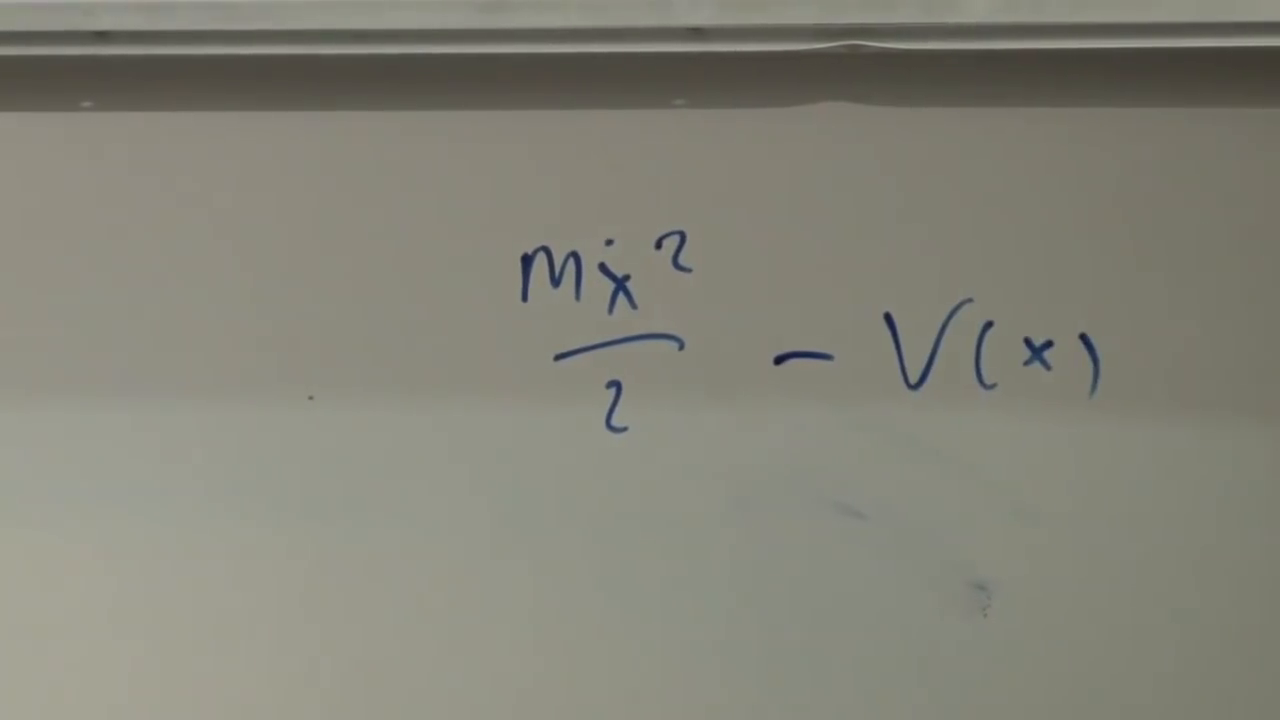
\includegraphics[width=0.72\textwidth]{lecture_04_figure_02.png} \caption{Lagrangian động năng trừ thế năng dùng để đồng nhất động lượng liên hợp với \(m\dot x\).} \lectureframe{00:14:48} \end{figure}

Nếu \(q_i\) không xuất hiện trong \(L\), thì \(\dot p_i=0\). Đây là con đường quen thuộc từ tọa độ tuần hoàn đến một định luật bảo toàn. Mối liên hệ thực sự thì tổng quát hơn, và sẽ hữu ích nếu nhận ra nó trong các ví dụ trước khi chứng minh nó.

\section{Các định luật bảo toàn được tìm ra trước khi được giải thích}

\subsection{Hai tọa độ và một thế năng theo độ tách}

Đặt cả hai khối lượng bằng 1 và lấy \begin{equation}
  L=\frac{\dot q_1^{\,2}+\dot q_2^{\,2}}{2}-V(q_1-q_2).
  \label{eq:separation-lagrangian}
\end{equation} Có thể hình dung hai hạt trên một đường thẳng. Tương tác của chúng chỉ phụ thuộc vào độ tách giữa chúng.

\begin{figure}[htbp] \centering
  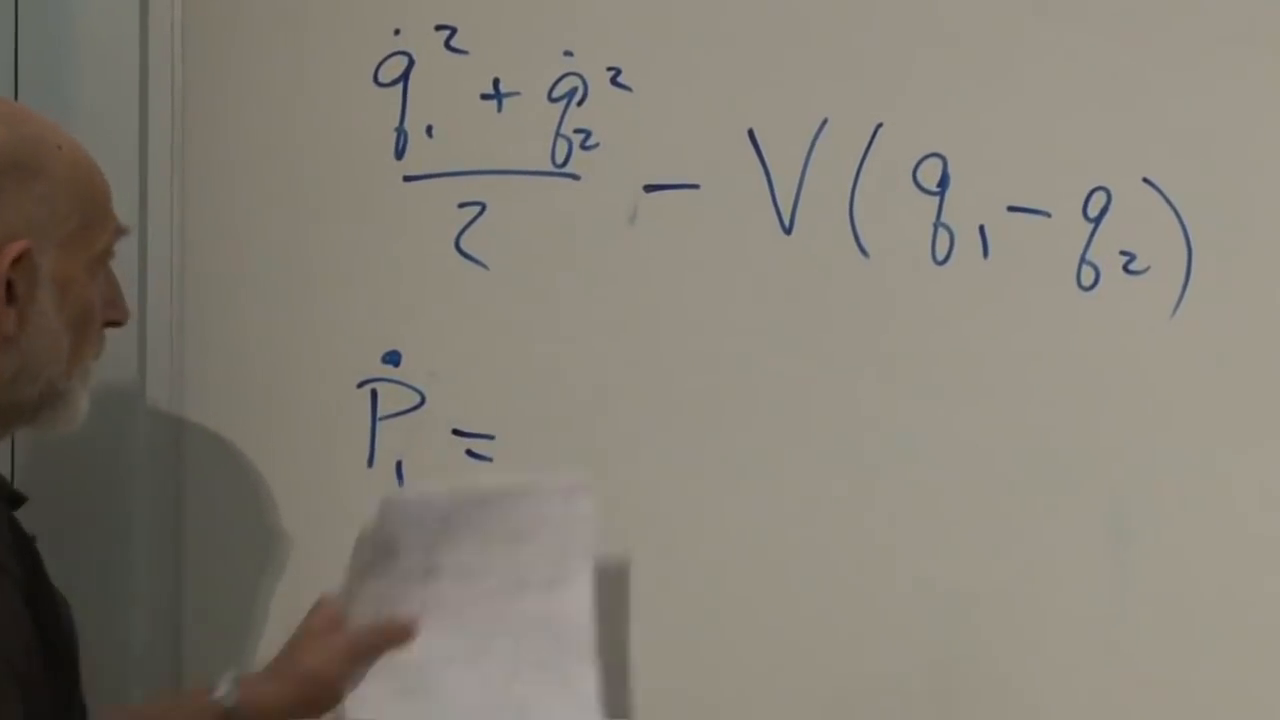
\includegraphics[width=0.78\textwidth]{lecture_04_figure_03.png} \caption{Lagrangian hai tọa độ và phần đầu của phương trình động lượng thứ nhất của nó.} \lectureframe{00:18:56} \end{figure}

Ký hiệu \(V'\) cho đạo hàm theo đối số của \(V\), \begin{align}
  \dot p_1&=-V'(q_1-q_2),
  \notag\\
  \dot p_2&=+V'(q_1-q_2).
  \label{eq:separation-momentum-equations}
\end{align} Dấu ở phương trình thứ hai đổi ngược vì tăng \(q_2\) làm giảm \(q_1-q_2\).

\begin{classroomqa} \audiencequestion{Phương trình động lượng thứ nhất có nên chứa \(V'\) không, và dấu trừ của nó từ đâu ra? \lecturetimestamp{00:20:52--00:21:35}} \lecturerresponse{Phương trình Euler--Lagrange nói \(\dot p_1=\partial L/\partial q_1\), chứ không phải Lagrangian bằng 0. Vì \(L=T-V\), nên khi đạo hàm theo \(q_1\) ta được \(-V'\). Lấy đạo hàm theo \(q_2\) đưa thêm vào một dấu trừ từ \(q_1-q_2\), nên phương trình thứ hai có \(+V'\).} \end{classroomqa}

\begin{figure}[htbp] \centering
  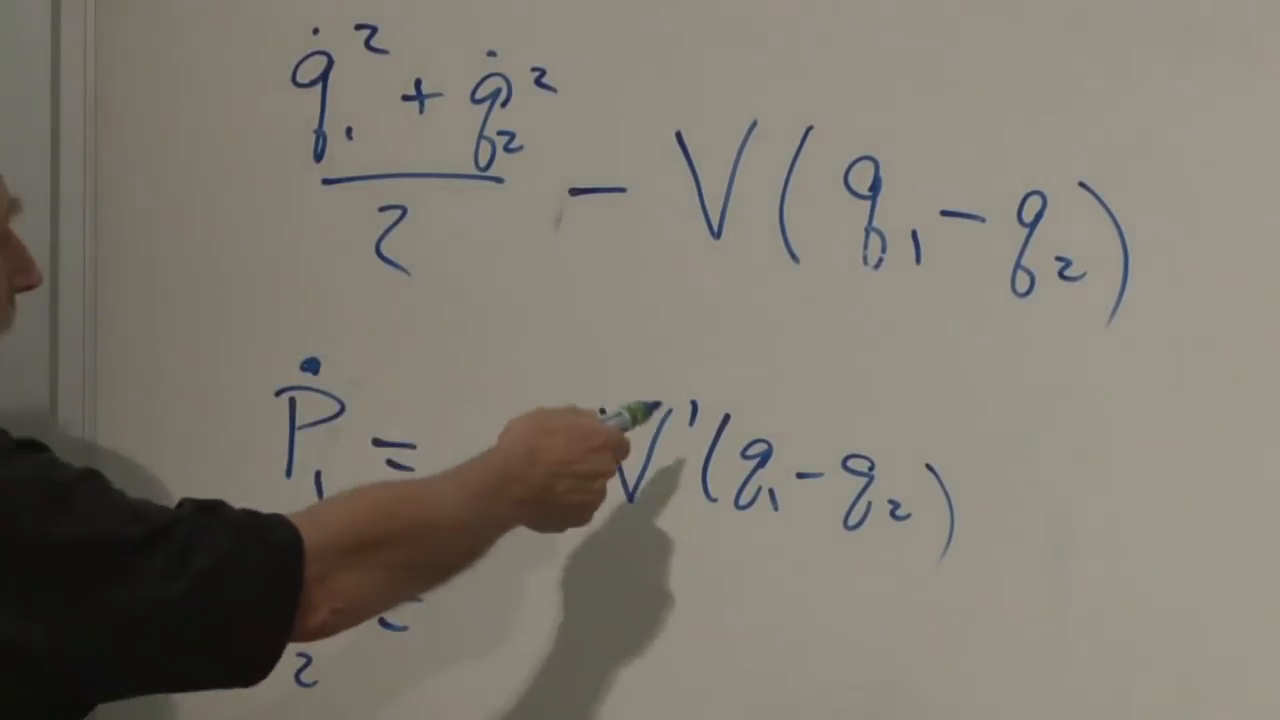
\includegraphics[width=0.78\textwidth]{lecture_04_figure_04.png} \caption{Đạo hàm nhạy với dấu trong phương trình \(p_1\); phương trình \(p_2\) nhận dấu ngược lại.} \lectureframe{00:20:41} \end{figure}

Cộng các phương trình ~\eqref{eq:separation-momentum-equations} ta được \begin{equation}
  \frac{d}{dt}(p_1+p_2)=0.
  \label{eq:total-p-conserved}
\end{equation} Ta đã tìm ra một đại lượng bảo toàn, nhưng vẫn chưa giải thích vì sao nó tồn tại.

\subsection{Một tổ hợp tuyến tính kém hiển nhiên hơn}

Bây giờ hãy lấy \begin{equation}
  L=\frac{\dot q_1^{\,2}+\dot q_2^{\,2}}{2}
    -V(Aq_1+Bq_2),
  \label{eq:ab-lagrangian}
\end{equation} trong đó \(A\) và \(B\) là các hằng số. Khi đó \begin{align}
  \dot p_1&=-A\,V'(Aq_1+Bq_2),
  \notag\\
  \dot p_2&=-B\,V'(Aq_1+Bq_2).
  \label{eq:ab-momentum-equations}
\end{align} Nhân phương trình thứ nhất với \(B\), phương trình thứ hai với \(A\), rồi lấy hiệu sẽ triệt tiêu lực: \begin{equation}
  \frac{d}{dt}(Bp_1-Ap_2)=0.
  \label{eq:ab-conserved}
\end{equation}

\begin{figure}[htbp] \centering
  \includegraphics[width=0.78\textwidth]{lecture_04_figure_06.png} \caption{Các phương trình động lượng có trọng số mà các hạng lực triệt tiêu trong \(Bp_1-Ap_2\).} \lectureframe{00:24:20} \end{figure}

\begin{classroomqa} \audiencequestion{Về mặt vật lý, các hằng số như \(A\) và \(B\) có thể đến từ đâu?\lecturetimestamp{00:25:09--00:30:15}} \lecturerresponse{Xét hai hạt có khối lượng \(m\) và \(M\): \[
    L=\frac{m\dot X^2}{2}+\frac{M\dot Y^2}{2}-V(X-Y).
  \] Đổi biến thành \(Q_1=\sqrt m\,X\) và \(Q_2=\sqrt M\,Y\). Khi đó hạng động năng trở thành \((\dot Q_1^2+\dot Q_2^2)/2\), còn thế năng phụ thuộc vào \(Q_1/\sqrt m-Q_2/\sqrt M\). Vì vậy, các khối lượng không bằng nhau tự nhiên trở thành các hệ số trong một tổ hợp tuyến tính. Thay \(Q_2\) bằng \(-Q_2\) sẽ biến dấu trừ đang viết thành dấu cộng mà không làm thay đổi hạng động năng bình phương của nó.} \end{classroomqa}

\begin{figure}[htbp] \centering
  \includegraphics[width=0.82\textwidth]{lecture_04_figure_07.png} \caption{Các tọa độ có trọng số khối lượng làm đơn giản động năng đồng thời đưa các thừa số khối lượng vào thế năng.} \lectureframe{00:28:40} \end{figure}

\begin{classroomqa} \audiencequestion{Điều này có cho thấy rằng một đại lượng bảo toàn có thể tồn tại mà không cần một tọa độ tuần hoàn không?\lecturetimestamp{00:31:13--00:31:58}} \lecturerresponse{Trong các biến như đã viết, không có tọa độ tuần hoàn \emph{hiển nhiên} nào. Một phép đổi biến có thể làm lộ ra một tọa độ như thế, nhưng việc truy tìm nó không phải là góc nhìn hữu ích ở đây. Lập luận đối xứng sẽ nhận diện trực tiếp tổ hợp được bảo toàn.} \end{classroomqa}

\section{Ta hiểu thế nào là một đối xứng}

\subsection{Phép tịnh tiến}

Bắt đầu với một hạt tự do khối lượng đơn vị, \begin{equation}
  L=\frac{\dot q^2}{2}.
  \label{eq:free-unit-l4}
\end{equation} Tịnh tiến toàn bộ lịch sử chuyển động của nó bởi cùng một hằng số: \begin{equation}
  q'(t)=q(t)+\epsilon.
  \label{eq:free-translation}
\end{equation} Vì \(\epsilon\) không phụ thuộc thời gian, \(\dot q'=\dot q\), và do đó \(\delta L=0\). Tính bất biến này là đối xứng tịnh tiến.

Có hai cách nhìn tương đương. Theo cách thụ động, ta dời gốc tọa độ trong khi giữ vật cố định. Theo cách chủ động, ta giữ cố định các trục và di chuyển vật. Cách nói chủ động sẽ tỏ ra ít gây nhầm lẫn hơn: hãy di chuyển cấu hình vật lý và hỏi xem \(L\) có thay đổi hay không.

Đối với phương trình ~\eqref{eq:separation-lagrangian}, hãy tịnh tiến cả hai tọa độ: \begin{equation}
  \delta q_1=\epsilon,
  \qquad
  \delta q_2=\epsilon.
  \label{eq:common-translation}
\end{equation} Các vận tốc không đổi và \(q_1-q_2\) cũng vậy.

\begin{figure}[htbp] \centering
  \includegraphics[width=0.78\textwidth]{lecture_04_figure_08.png} \caption{Phép tịnh tiến đồng thời giữ nguyên độ tách giữa hai tọa độ.} \lectureframe{00:35:30} \end{figure}

Đối với phương trình ~\eqref{eq:ab-lagrangian}, hãy dùng phép biến đổi kém hiển nhiên hơn \begin{equation}
  \delta q_1=B\epsilon,
  \qquad
  \delta q_2=-A\epsilon.
  \label{eq:ab-transformation}
\end{equation} Một lần nữa, các vận tốc không đổi, còn \begin{equation}
  \delta(Aq_1+Bq_2)=AB\epsilon-BA\epsilon=0.
  \label{eq:ab-invariant-argument}
\end{equation} Vì vậy phép biến đổi này là một đối xứng.

\begin{figure}[htbp] \centering
  \includegraphics[width=0.80\textwidth]{lecture_04_figure_09.png} \caption{Phép tịnh tiến bất đối xứng giữ nguyên \(Aq_1+Bq_2\).} \lectureframe{00:40:20} \end{figure}

\begin{classroomqa} \audiencequestion{Các hệ số ấy có mã hóa khối lượng hay không, để đại lượng bảo toàn trở thành động lượng khối tâm thông thường? \lecturetimestamp{00:42:25--00:42:45}} \lecturerresponse{Có. Trong các biến có trọng số khối lượng, đối xứng và tổ hợp bảo toàn trông bất đối xứng. Biến đổi ngược về \(X\) và \(Y\) sẽ phục hồi phép tịnh tiến đồng thời thông thường và tổng động lượng.} \end{classroomqa}

\subsection{Phép quay}

Hãy xét một hạt trong mặt phẳng, \begin{equation}
  L=\frac{m}{2}(\dot x^2+\dot y^2)-V(x^2+y^2).
  \label{eq:central-lagrangian-l4}
\end{equation} Đây là một thế năng tâm. Ta so sánh hai hệ tọa độ cố định lệch nhau bởi một phép quay; các trục không quay theo thời gian. Với một quy ước định hướng nhất quán, \begin{align}
  x'&=x\cos\theta+y\sin\theta,
  \notag\\
  y'&=-x\sin\theta+y\cos\theta.
  \label{eq:finite-rotation-l4}
\end{align}

\begin{figure}[htbp] \centering
  \includegraphics[width=0.82\textwidth]{lecture_04_figure_10.png} \caption{Một Lagrangian thế năng tâm và hai hệ Descartes cố định liên hệ với nhau bởi một phép quay.} \lectureframe{00:45:40} \end{figure}

Đặt \(\theta=\epsilon\) và chỉ giữ đến bậc nhất: \begin{equation}
  \cos\epsilon=1+O(\epsilon^2),
  \qquad
  \sin\epsilon=\epsilon+O(\epsilon^3).
  \label{eq:small-angle-l4}
\end{equation} Phép quay vô cùng bé là \begin{align}
  \delta x&=y\epsilon,
  &\delta y&=-x\epsilon,
  \notag\\
  \delta\dot x&=\dot y\epsilon,
  &\delta\dot y&=-\dot x\epsilon.
  \label{eq:infinitesimal-rotation-l4}
\end{align}

\begin{figure}[htbp] \centering
  \includegraphics[width=0.82\textwidth]{lecture_04_figure_11.png} \caption{Phép quay vô cùng bé của các tọa độ và vận tốc.} \lectureframe{00:49:50} \end{figure}

Không như trong phép tịnh tiến, độ lớn thay đổi của \(x\) phụ thuộc vào \(y\), còn độ lớn thay đổi của \(y\) phụ thuộc vào \(x\). Tuy vậy, \begin{align}
  \delta(x^2+y^2)
  &=2x\,\delta x+2y\,\delta y=0,
  \notag\\
  \delta(\dot x^2+\dot y^2)
  &=2\dot x\,\delta\dot x+2\dot y\,\delta\dot y=0.
  \label{eq:rotation-invariants-l4}
\end{align} Cả hạng thế năng lẫn hạng động năng đều bất biến.

\begin{figure}[htbp] \centering
  \includegraphics[width=0.76\textwidth]{lecture_04_figure_12.png} \caption{Sự triệt tiêu ở bậc nhất chứng minh rằng bình phương bán kính bất biến dưới phép quay.} \lectureframe{00:53:20} \end{figure}

\section{Định lý bảo toàn tổng quát}

Các ví dụ về tịnh tiến và quay có chung một dạng. Hãy xét một phép biến đổi vô cùng bé liên tục \begin{equation}
  \delta q_i=\epsilon f_i(q),
  \qquad
  \delta\dot q_i=\frac{d}{dt}\delta q_i,
  \label{eq:general-infinitesimal-symmetry}
\end{equation} trong đó \(\epsilon\) không phụ thuộc thời gian và \(f_i\) có thể phụ thuộc vào mọi tọa độ.

\begin{figure}[htbp] \centering
  \includegraphics[width=0.78\textwidth]{lecture_04_figure_13.png} \caption{Một trường độ dời vô cùng bé tổng quát \(\delta q_i=\epsilon f_i(q)\).} \lectureframe{00:56:00} \end{figure}

Biến thiên bậc nhất của Lagrangian là \begin{equation}
  \delta L
  =\sum_i\left(
    \frac{\partial L}{\partial q_i}\delta q_i
    +\frac{\partial L}{\partial\dot q_i}\delta\dot q_i
  \right).
  \label{eq:delta-l-general}
\end{equation}

\begin{figure}[htbp] \centering
  \includegraphics[width=0.84\textwidth]{lecture_04_figure_14.png} \caption{Hai đóng góp vào \(\delta L\): biến thiên tọa độ và biến thiên vận tốc.} \lectureframe{01:02:30} \end{figure}

Bây giờ hãy giới hạn sự chú ý vào một quỹ đạo vật lý, để các phương trình Euler--Lagrange được thỏa mãn. Dùng \begin{equation}
  \frac{\partial L}{\partial\dot q_i}=p_i,
  \qquad
  \frac{\partial L}{\partial q_i}=\dot p_i,
  \label{eq:el-substitution-l4}
\end{equation} ta tìm được \begin{align}
  \delta L
  &=\sum_i\left(\dot p_i\,\delta q_i
                +p_i\,\delta\dot q_i\right)
  \notag\\
  &=\frac{d}{dt}\sum_i p_i\delta q_i
  =\epsilon\frac{d}{dt}\sum_i p_i f_i(q).
  \label{eq:noether-derivation-l4}
\end{align} Bước mấu chốt chỉ là quy tắc tích.

Nếu phép biến đổi là một đối xứng, thì \(\delta L=0\). Vì \(\epsilon\) là một thừa số hằng tùy ý, \begin{equation}
  \boxed{
  \frac{d\mathcal Q}{dt}=0,
  \qquad
  \mathcal Q=\sum_i p_i f_i(q)}
  .
  \label{eq:noether-charge-l4}
\end{equation} Đây là phần cốt lõi trong cơ học cổ điển của định lý Noether đối với các đối xứng điểm chính xác, không phụ thuộc thời gian.

\begin{figure}[htbp] \centering
  \includegraphics[width=0.84\textwidth]{lecture_04_figure_15.png} \caption{Bước dùng quy tắc tích biến tính bất biến của \(L\) thành một đại lượng bảo toàn.} \lectureframe{01:05:00} \end{figure}

\begin{classroomqa} \audiencequestion{Trong \(f_i(q)\), \(q\) có mang thêm một chỉ số nữa không? \lecturetimestamp{01:06:57--01:07:31}} \lecturerresponse{Ký hiệu \(q\) không gắn chỉ số biểu thị toàn bộ tập \((q_1,q_2,\ldots)\). Mỗi thành phần \(f_i\) có thể phụ thuộc vào toàn bộ các tọa độ đó. Chẳng hạn, đối với phép quay, \(f_x=y\) và \(f_y=-x\).} \end{classroomqa}

Các ví dụ giờ đây không còn là ngẫu nhiên nữa. Một phép tịnh tiến đồng thời có \(f_1=f_2=1\), nên \begin{equation}
  \mathcal Q=p_1+p_2.
  \label{eq:noether-common-p}
\end{equation} Phép tịnh tiến bất đối xứng có \(f_1=B\), \(f_2=-A\), nên \begin{equation}
  \mathcal Q=Bp_1-Ap_2.
  \label{eq:noether-ab-p}
\end{equation} Với phép quay, \(f_x=y\) và \(f_y=-x\): \begin{equation}
  \mathcal Q=p_xy-p_yx.
  \label{eq:rotation-charge-sign}
\end{equation} Sai khác ở một dấu do định hướng, đây là mômen động lượng, \begin{equation}
  J=xp_y-yp_x.
  \label{eq:angular-momentum-l4}
\end{equation}

\begin{figure}[htbp] \centering
  \includegraphics[width=0.82\textwidth]{lecture_04_figure_16.png} \caption{Đại lượng Noether của phép quay, sai khác với mômen động lượng trong mặt phẳng bởi một dấu định hướng.} \lectureframe{01:11:00} \end{figure}

Đối với nhiều hạt tương tác, hãy quay tất cả các hạt cùng nhau. Khi đó tính bất biến bảo toàn tổng các mômen động lượng của chúng, chứ không bảo toàn riêng rẽ mômen động lượng của từng hạt.

\section{Những câu hỏi về các giả thiết của định lý}

\begin{classroomqa} \audiencequestion{Một hệ trục quay có đưa sự phụ thuộc thời gian tường minh vào \(\delta L\) hay không?\lecturetimestamp{01:12:57--01:13:57}} \lecturerresponse{Có. Chứng minh vừa nêu giả sử tham số đối xứng không phụ thuộc thời gian: một phép tịnh tiến cố định hoặc một phép quay cố định. Một phép biến đổi có tham số phụ thuộc thời gian sẽ sinh thêm các hạng và đòi hỏi một cách xử lý tổng quát hơn.} \end{classroomqa}

\begin{classroomqa}
  \audiencequestion{Chữ hoa \(Q\) trong công thức trên bảng có phải là chính phép biến đổi không?\lecturetimestamp{01:14:02--01:15:58}}
  \lecturerresponse{Không. Ký hiệu đó không may bị trùng với các tọa độ \(q_i\). Phép biến đổi là \(\delta q_i=\epsilon f_i(q)\); đại lượng bảo toàn thu được là \(\mathcal Q=\sum_i p_i f_i\). Hệ số \(f_i\) cho biết tọa độ thứ \(i\) dịch chuyển như thế nào dưới đối xứng ấy.}
\end{classroomqa}

Bảo toàn năng lượng cũng được sinh ra bởi một đối xứng, nhưng là một đối xứng khác: phép tịnh tiến theo thời gian, hay tính độc lập đối với việc đặt mốc không của thời gian ở đâu. Trường hợp đó và dạng thức Hamilton được để lại xét sau.

\begin{classroomqa}
  \audiencequestion{Liệu chuyển động thực có thể được hấp thụ vào một hệ tọa độ đang thay đổi, để cơ học trở thành chẳng qua chỉ là các phép biến đổi tọa độ?\lecturetimestamp{01:17:43--01:20:01}}
  \lecturerresponse{Người ta có thể chọn các tọa độ đi theo một chuyển động cụ thể, nhưng khi đó phép biến đổi phụ thuộc vào trạng thái ban đầu và vào quỹ đạo. Phép biến đổi đối xứng được dùng ở đây là cố định, độc lập với việc hệ đi theo nghiệm nào. Bản thân chuyển động được biểu diễn tự nhiên hơn trong không gian kết hợp của tọa độ và xung lượng.}
\end{classroomqa}

\section{Dao động điều hòa trong không gian pha}

Với khối lượng và hằng số lò xo đều được đặt bằng một,
\begin{equation}
  L=\frac{\dot q^2}{2}-\frac{q^2}{2}.
  \label{eq:oscillator-l4}
\end{equation}
Xung lượng liên hợp và phương trình chuyển động cho
\begin{equation}
  p=\dot q,
  \qquad
  \dot p=-q,
  \label{eq:oscillator-first-order-l4}
\end{equation}
hoặc
\begin{equation}
  \dot q=p,
  \qquad
  \dot p=-q.
  \label{eq:oscillator-phase-flow}
\end{equation}
Các phương trình này mô tả chuyển động tròn đều trong mặt phẳng \(q\)-\(p\).
Dao động tử qua lại trong không gian thực là hình chiếu của đường tròn đó lên trục \(q\): độ lớn vận tốc lớn nhất tại \(q=0\) và triệt tiêu ở các điểm đổi chiều.

\begin{figure}[htbp]
  \centering
  \includegraphics[width=0.82\textwidth]{lecture_04_figure_17.png}
  \caption{Các phương trình của dao động điều hòa và quỹ đạo tròn của nó trong không gian \(q\)-\(p\).}
  \lectureframe{01:25:30}
\end{figure}

\begin{classroomqa}
  \audiencequestion{Đường tròn trong không gian pha có chạy theo chiều kim đồng hồ không?
  \lecturetimestamp{01:25:47--01:27:15}}
  \lecturerresponse{Nếu \(p\) nằm ngang và \(q\) thẳng đứng, thì có. Tại \(q\) dương cực đại, \(\dot p=-q<0\), nên chuyển động hướng xuống dưới. Đảo cách đặt các trục sẽ đảo ngược cảm nhận thị giác ấy, điều này giải thích vì sao rất dễ nhớ nhầm quy ước.}
\end{classroomqa}

Cặp phương trình trong Eq.~\eqref{eq:oscillator-phase-flow} đã khá giống các phương trình Hamilton, nhưng nó được suy ra hoàn toàn trong khuôn khổ cơ học Lagrange.

\section{Các đối xứng liên tục và rời rạc}

\begin{classroomqa}
  \audiencequestion{Một đối xứng có nhất thiết phải được biểu diễn bằng một phép biến đổi Cartesian vô cùng bé không?\lecturetimestamp{01:27:48--01:30:31}}
  \lecturerresponse{Tọa độ Cartesian chỉ là thuận tiện; yêu cầu cốt yếu đối với chứng minh này là tính liên tục. Một số đối xứng không có phiên bản vô cùng bé. Với một thế chẵn, phép phản xạ biến \(q\mapsto -q\) và \(\dot q\mapsto-\dot q\), giữ \(L\) không đổi, nhưng một phép phản xạ không thể được ghép từ các phép phản xạ nhỏ đến tùy ý. Vì thế, suy dẫn cổ điển này không tạo ra đại lượng bảo toàn liên hệ nào.}
\end{classroomqa}

\begin{figure}[htbp]
  \centering
  \includegraphics[width=0.82\textwidth]{lecture_04_figure_18.png}
  \caption{Một thế chẵn là bất biến dưới phép phản xạ rời rạc \(q\mapsto -q\).}
  \lectureframe{01:29:30}
\end{figure}

\begin{classroomqa}
  \audiencequestion{Nếu đại lượng bảo toàn \(\mathcal Q\) khác không, điều đó có cho thấy phép biến đổi đã không phải là một đối xứng không?
  \lecturetimestamp{01:30:40--01:31:30}}
  \lecturerresponse{Không. Một đại lượng bảo toàn có thể nhận bất kỳ giá trị hằng nào. Tiêu chuẩn liên quan là \(\dot{\mathcal Q}\). Nếu đại lượng rút ra từ một phép biến đổi được đề xuất không được bảo toàn, thì dưới các giả thiết của chứng minh, phép biến đổi được đề xuất đó không phải là đối xứng.}
\end{classroomqa}

\begin{classroomqa}
  \audiencequestion{Phản xạ vẫn giữ Lagrangian không đổi, vậy tại sao lại không có định luật bảo toàn nào từ nó?\lecturetimestamp{01:31:34--01:32:27}}
  \lecturerresponse{Riêng tính bất biến thì thấy được, nhưng phép suy dẫn đã đi qua một độ dời bậc nhất và quy tắc tích. Phản xạ đưa một phía của không gian cấu hình sang phía bên kia trong một bước rời rạc duy nhất. Không có bộ sinh vô cùng bé \(f_i\), công thức \(\mathcal Q=\sum_i p_i f_i\) không có gì để dùng.}
\end{classroomqa}

\begin{classroomqa}
  \audiencequestion{Tên gọi của tính chất có thể được ghép từ các phép biến đổi nhỏ đến tùy ý là gì?\lecturetimestamp{01:32:36--01:33:23}}
  \lecturerresponse{Đó là một \emph{đối xứng liên tục}. Phép tịnh tiến và phép quay là liên tục; phản xạ là một \emph{đối xứng rời rạc}.}
\end{classroomqa}

\begin{classroomqa}
  \audiencequestion{Nếu nhiều bước vô cùng bé tạo thành một phép biến đổi hữu hạn, các sai số \(O(\epsilon^2)\) bị bỏ đi có thể tích lũy không?
  \lecturetimestamp{01:33:23--01:36:10}}
  \lecturerresponse{Tính bất biến vô cùng bé phải đúng tại mọi điểm đạt tới dọc theo phép biến đổi, chứ không chỉ ở điểm xuất phát. Chia một khoảng tham số hữu hạn thành \(N\) bước có kích thước \(\epsilon\): độ dời bậc nhất tích lũy là \(N\epsilon\), còn phần dư cục bộ \(O(\epsilon^2)\) tích lũy thành \(N\epsilon^2=(N\epsilon)\epsilon\to0\). Đây là cấu trúc từ cục bộ đến hữu hạn được hình thức hóa bởi các nhóm biến đổi liên tục.}
\end{classroomqa}

\begin{classroomqa}
  \audiencequestion{Các đối xứng rời rạc có được hiện thực hóa về mặt vật lý trong các hệ cổ điển không?\lecturetimestamp{01:36:32--01:37:25}}
  \lecturerresponse{Chắc chắn có. Chính dao động điều hòa có thế chẵn \(V(q)\propto q^2\), nên nó bất biến dưới \(q\mapsto -q\). Có nhiều ví dụ như vậy; điểm ở đây chỉ là tính bất biến rời rạc này không cung cấp đại lượng bảo toàn Noether cổ điển mới nào.}
\end{classroomqa}

\begin{classroomqa}
  \audiencequestion{Nhưng nếu cả các phép biến đổi liên tục lẫn rời rạc đều giữ \(L\) không đổi, chẳng phải đó là cùng một điều kiện sao?
  \lecturetimestamp{01:37:37--01:39:18}}
  \lecturerresponse{Đó là cùng một phát biểu hữu hạn về tính bất biến, nhưng không phải là cùng một đầu vào toán học cho chứng minh này. Chứng minh cần một biến thiên bậc nhất. Với phản xạ, 'bậc nhất' không có nghĩa, nên chuỗi phương trình dẫn đến một đại lượng bảo toàn thậm chí còn không thể bắt đầu.}
\end{classroomqa}

\begin{classroomqa}
  \audiencequestion{Về mặt lịch sử, điều này liên hệ thế nào với định lý Noether?\lecturetimestamp{01:39:26--01:40:42}}
  \lecturerresponse{Đây là một phần hạn chế của định lý tổng quát hơn rất nhiều của Emmy Noether. Những mối liên hệ cụ thể giữa đối xứng và các đại lượng bảo toàn đã được biết đến từ trước, nhưng Noether đã đặt chúng vào một khuôn khổ thống nhất và đặc biệt tổng quát vào đầu thế kỷ XX. Tầm quan trọng toán học của bà đã không được đối xử công bằng tương xứng trong giới học thuật.}
\end{classroomqa}

\begin{classroomqa}
  \audiencequestion{Cơ học cổ điển vẫn còn là một chủ đề nghiên cứu đang hoạt động chứ?\lecturetimestamp{01:40:47--01:42:37}}
  \lecturerresponse{Có. Định lý sơ cấp được dùng ở đây đã lâu đời, nhưng động lực học phi tuyến, các hệ khả tích, hỗn loạn, chất lưu và cơ học hình học vẫn là những lĩnh vực phong phú. Nguyên lý đối xứng cũng còn tiếp tục vượt xa cơ học hạt cổ điển.}
\end{classroomqa}

\section{Vì sao nguyên lý tác dụng lại quan trọng}

\begin{classroomqa}
  \audiencequestion{Có lý do trực giác nào để đối xứng phải kéo theo bảo toàn không?\lecturetimestamp{01:42:49--01:47:57}}
  \lecturerresponse{Không phải chỉ từ riêng đối xứng. Hãy xét lực cản nhớt,
  \[
    m\ddot x=-c\dot x.
  \]
  Phương trình này bất biến dưới \(x\mapsto x+\epsilon\), nhưng với
  \(p=m\dot x\),
  \[
    \dot p=-\frac{c}{m}p,
    \qquad
    p(t)=p(0)e^{-ct/m},
  \]
  nên xung lượng suy giảm. Đây là một phương trình hiệu dụng cho một phân hệ, chứ không phải một định luật cơ bản theo nguyên lý tác dụng dừng cho riêng \(x\). Nếu kể cả các phân tử chất lỏng và phần còn lại của hệ kín, thì tổng xung lượng được bảo toàn. Đối xứng và bảo toàn gắn với nhau thông qua nguyên lý tác dụng Lagrangian, chứ không phải chỉ qua sự xuất hiện của bản thân một phương trình vi phân.}
\end{classroomqa}

\begin{figure}[htbp]
  \centering
  \includegraphics[width=0.65\textwidth]{lecture_04_figure_19.png}
  \caption{Lực cản nhớt bất biến đối với tịnh tiến, nhưng xung lượng của hạt trong mô tả rút gọn vẫn suy giảm.}
  \lectureframe{01:44:30}
\end{figure}

\begin{classroomqa}
  \audiencequestion{Ta có thể lượng hóa khi nào quỹ đạo vật lý không phải là cực tiểu của tác dụng không?\lecturetimestamp{01:48:08--01:51:38}}
  \lecturerresponse{Một cực tiểu thực sự là trường hợp ngoại lệ; nói chung tác dụng là một điểm yên ngựa trong không gian các quỹ đạo. Đối với dao động tử đơn vị,
  \[
    S[q]=\frac12\int(\dot q^2-q^2)\,dt.
  \]
  Một biến dạng hẹp, biến thiên nhanh làm tăng đóng góp dương \(\dot q^2\). Một biến dạng rộng, duy trì độ lệch nhỏ trong một thời gian dài, có thể làm cho đóng góp âm \(-q^2\) lấn át và hạ thấp tác dụng. Vì vậy cùng một quỹ đạo dừng vừa có những hướng làm tăng vừa có những hướng làm giảm. Cơ học lượng tử, thông qua quan điểm tích phân đường đi, cho nguồn gốc sâu hơn của tính dừng, nhưng lập luận đó được để lại xét sau.}
\end{classroomqa}

\begin{figure}[htbp]
  \centering
  \includegraphics[width=0.80\textwidth]{lecture_04_figure_20.png}
  \caption{Một quỹ đạo dao động tử lân cận nhưng rộng minh họa vì sao tác dụng dừng điển hình là một điểm yên ngựa hơn là một cực tiểu.}
  \lectureframe{01:50:20}
\end{figure}

\begin{classroomqa}
  \audiencequestion{Có sự tương ứng một-một giữa các đối xứng liên tục và các định luật bảo toàn không?\lecturetimestamp{01:51:44--01:52:43}}
  \lecturerresponse{Trong khuôn khổ biến phân, và sau khi đồng nhất các trường hợp tương đương hoặc tầm thường, thì về cơ bản đó là bức tranh đúng. Mỗi đối xứng liên tục có một đại lượng Noether, và các đại lượng bảo toàn nói chung có thể được liên hệ ngược lại với các đối xứng. Các phát biểu chính xác có kèm những điều kiện kỹ thuật, nên không nên dùng phát biểu khái quát ấy một cách cẩu thả.}
\end{classroomqa}

\begin{classroomqa}
  \audiencequestion{Mọi Lagrangian có nhất thiết phải có một đối xứng không tầm thường không?\lecturetimestamp{01:52:43--01:53:23}}
  \lecturerresponse{Không. Các ví dụ đã được chọn sao cho có đối xứng. Một Lagrangian tổng quát không nhất thiết bất biến dưới bất kỳ phép biến đổi không gian nào được đề xuất.}
\end{classroomqa}

\begin{classroomqa}
  \audiencequestion{Cuối cùng, nên hiểu một đối xứng là một phép dời chủ động hay một sự đổi tọa độ thụ động?
  \lecturetimestamp{01:53:25--01:55:08}}
  \lecturerresponse{Cả hai cách mô tả đều có thể được làm cho tương đương, nhưng ở đây cách chủ động sáng sủa hơn. Hãy dời toàn bộ hệ vật lý và hỏi xem Lagrangian có thay đổi hay không. Trong ngôn ngữ thụ động, thay vào đó phải nói rằng \emph{dạng} của Lagrangian không đổi khi hệ quy chiếu tọa độ dịch chuyển.}
\end{classroomqa}

\begin{classroomqa}
  \audiencequestion{Tiếp theo là gì?\lecturetimestamp{01:55:10--01:55:35}}
  \lecturerresponse{Bảo toàn năng lượng, nguồn gốc của nó trong đối xứng tịnh tiến theo thời gian, rồi đến dạng thức Hamilton.}
\end{classroomqa}